\chapter{Context}
\label{chap:contexte}

\section{The host organisation}

\subsection{Field of activity}
The UCAC-ICAM Institute is a Cameroonian higher-education institution located in Douala. It is attached to the Catholic University of Central Africa (UCAC, headquartered in Yaoundé), whose academic direction is entrusted to ICAM (Institut Catholique d'Arts et Métiers), a group of French engineering schools. Its main mission is to train, in Africa and for Africa, technicians and engineers who are professionally competent and humanly responsible, by combining theoretical knowledge with practice in the field.

The Institute operates in the CEMAC zone (Cameroon, Congo, Gabon, Central African Republic, Chad) and meets the needs of the sub-region's companies by training engineers and technicians who are operational from graduation. It has about 58 staff members, split between teaching, administrative and technical support staff, which allows close supervision of students. Its main ``customers'' are the students and their families, as well as the partner companies that host its interns and apprentices and recruit its graduates.

To date, the Institute reports more than 1000 graduated engineers and technicians, more than 800 apprenticeship contracts, more than 329 industrial missions, and two campuses: Douala (Cameroon) and Pointe-Noire (Republic of the Congo).

\subsection{History}
The Institute was founded in 2002 in Pointe-Noire (Republic of the Congo) as part of the partnership between UCAC and ICAM, before opening its Douala campus in 2004. The Douala campus first welcomed students from Pointe-Noire for the second cycle of the general engineering programme, then the computer engineering programme from 2015 and the general engineering programme with an international and innovation track from 2018. Over the years, the Institute has built international partnerships opening double-degree possibilities, notably with CESI École d'Ingénieurs (France) and the University of Sherbrooke (Canada).

\subsection{Fact sheet}
\begin{table}[h]
\centering
\renewcommand{\arraystretch}{1.25}
\begin{tabularx}{\textwidth}{|>{\bfseries\columncolor{ucacred!8}}l|X|}
\hline
Name & UCAC-ICAM Institute, Douala campus \\
\hline
Legal status & Private higher-education institution (Catholic University of Central Africa) \\
\hline
Address & Yansoki, near Yassa, Douala, Cameroon \\
\hline
Phone & (+237) 243 11 13 96 \\
\hline
Email & info.dla@ucac-icam.com \\
\hline
Website & \href{https://www.ucac-icam.com}{www.ucac-icam.com} \\
\hline
Field of activity & Training of engineers and technicians \\
\hline
\end{tabularx}
\caption{Fact sheet of the host organisation}
\end{table}

\subsection{Staff and programmes}
The Institute's staff is divided into two poles: training and administration (Table~\ref{tab:personnel}). Figures~\ref{fig:org-douala} and~\ref{fig:org-pointe-noire} show the management teams of the Douala and Pointe-Noire campuses.

\begin{table}[h]
\centering
\renewcommand{\arraystretch}{1.2}
\begin{tabularx}{\textwidth}{|l|p{4.3cm}|X|}
\hline
\rowcolor{ucacred!15} \textbf{Pole} & \textbf{Function} & \textbf{Role} \\
\hline
\multirow{4}{*}{Training} & Director of studies & Responsible for academic programmes and for steering teaching orientations \\
\cline{2-3}
 & Programme coordinators & Each one is in charge of a specific programme (computer science, general engineering by apprenticeship, innovation and entrepreneurship, process engineering) \\
\cline{2-3}
 & Year tutors and deputy tutors & Support students throughout their studies and ensure academic follow-up \\
\cline{2-3}
 & Lecturers (visiting and tutors) & Deliver theoretical and practical teaching according to their expertise \\
\hline
\multirow{5}{*}{Administration} & Director of the Institute & Responsible for organisation, vision and strategic development \\
\cline{2-3}
 & Finance department & Management of finances, budgets and financial resources \\
\cline{2-3}
 & Higher-education department & Administrative coordination of teaching and academic management \\
\cline{2-3}
 & Communication department & Internal and external communication, visibility and reputation \\
\cline{2-3}
 & Company relations department & Management of partnerships with companies, internships and collaborations \\
\hline
\end{tabularx}
\caption{Organisation of the Institute's staff}
\label{tab:personnel}
\end{table}

\begin{figure}[!htbp]
\centering
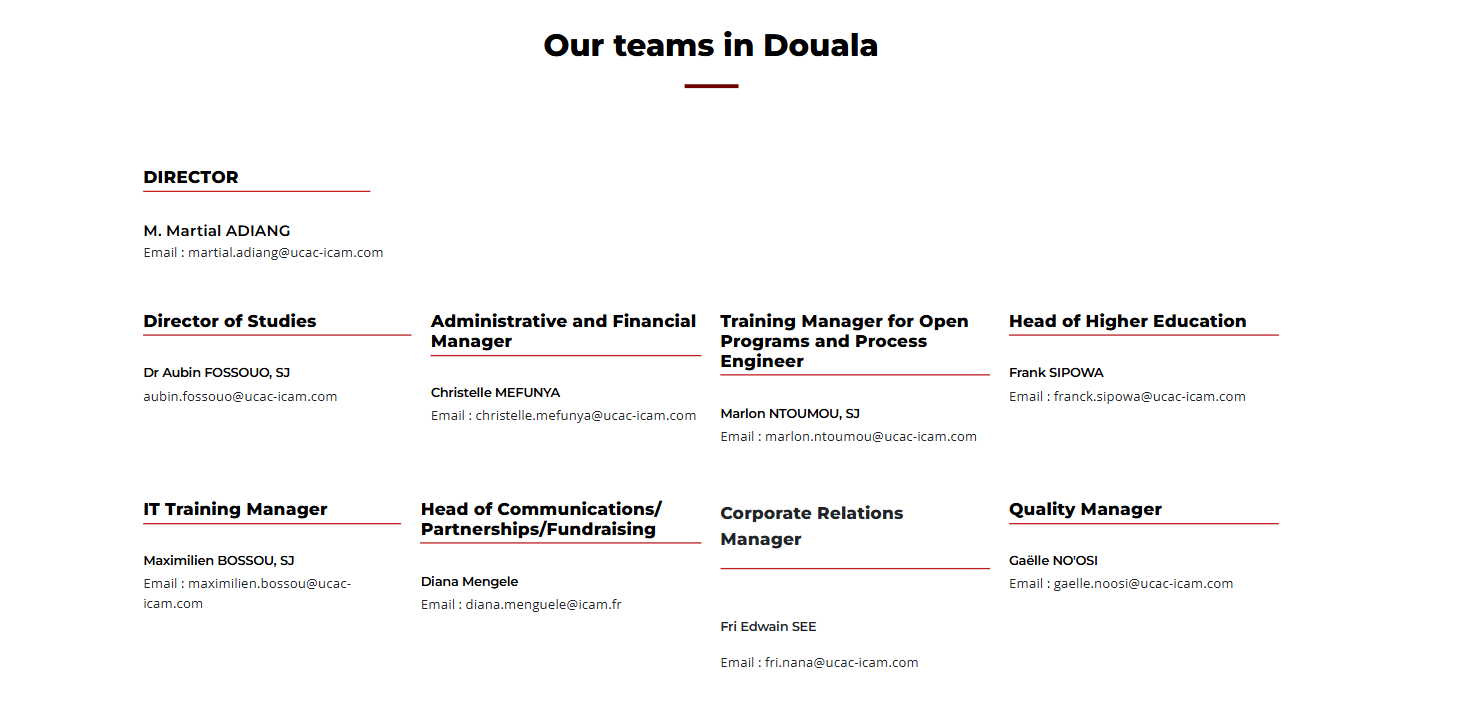
\includegraphics[width=\textwidth]{organigramme-douala.png}
\caption{Staff chart of the UCAC-ICAM Institute, Douala (source: the Institute's website, ``Our teams'' section).}
\label{fig:org-douala}
\end{figure}

\begin{figure}[!htbp]
\centering
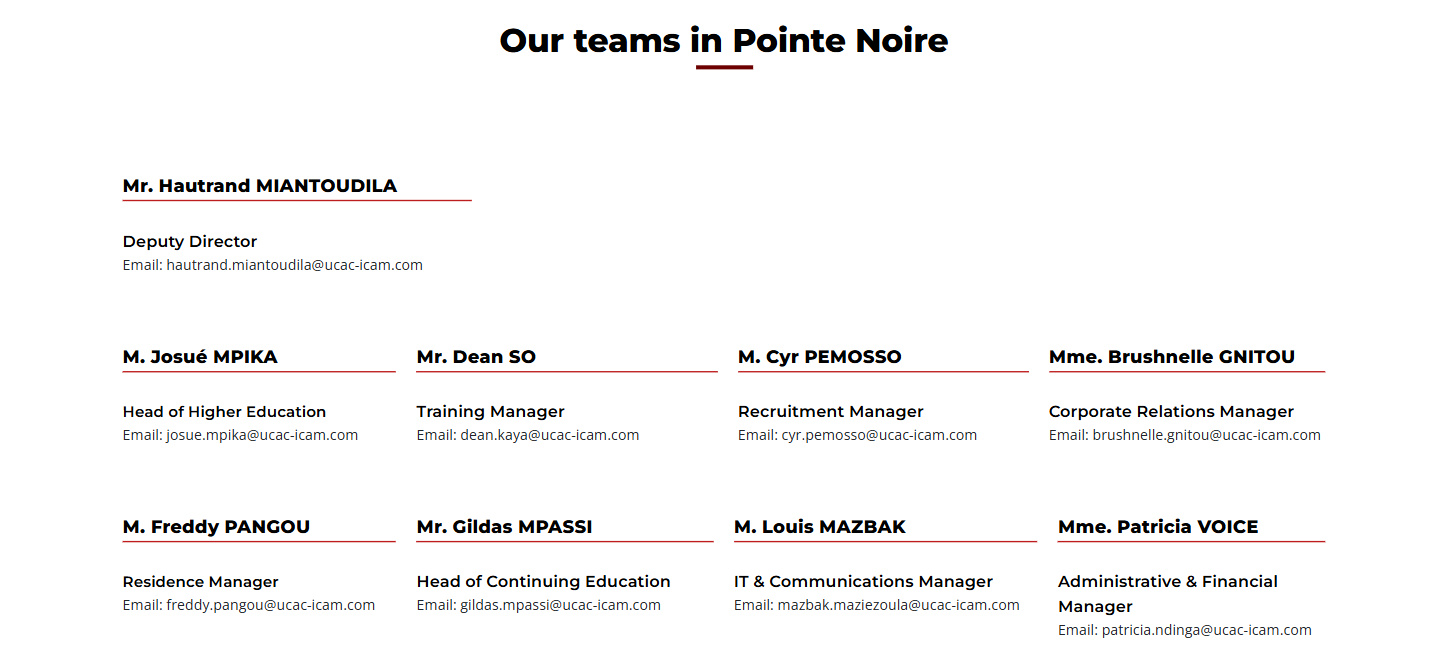
\includegraphics[width=\textwidth]{organigramme-pointe-noire.png}
\caption{Staff chart of the UCAC-ICAM Institute, Pointe-Noire (source: the Institute's website, ``Our teams'' section).}
\label{fig:org-pointe-noire}
\end{figure}

The Institute offers four main programmes, split into five training courses identified by a code (Table~\ref{tab:filieres}). My class, X2028, belongs to the computer engineering programme (code X); X4 designates its fourth year.

\begin{table}[h]
\centering
\renewcommand{\arraystretch}{1.15}
\begin{tabularx}{\textwidth}{|c|p{3.3cm}|X|}
\hline
\rowcolor{ucacred!15} \textbf{Code} & \textbf{Programme} & \textbf{Content} \\
\hline
X & Computer engineering & IT infrastructure management, data science and analysis, cybersecurity and software engineering. \\
\hline
A & General engineering, by apprenticeship & Interdisciplinary programme with a practical approach and immersion in an industrial company. \\
\hline
O & General engineering, international track & Same foundation as programme A, with international immersion in partner universities. \\
\hline
I & Innovation and entrepreneurship & Engineers able to lead innovative projects, with an emphasis on creativity, sustainability and entrepreneurship. \\
\hline
IP & Process engineering & Optimisation of production processes within environmental and energy constraints. \\
\hline
\end{tabularx}
\caption{Programmes and training courses of the Institute}
\label{tab:filieres}
\end{table}

\subsection{The IT department}
The IT department of the Douala campus administers the Institute's internal network, hosts and maintains the applications used by the various services, and provides technical support to staff. It is headed by Fr. Maximilien Bossou. Figure~\ref{fig:organigramme} shows my position within it; the diagram only shows the reporting line relevant to this internship, not the Institute's full organisation chart.

\begin{figure}[h]
\centering
\begin{tikzpicture}[
  box/.style={draw, thick, rounded corners=1pt, minimum height=0.9cm, minimum width=5cm, align=center, font=\small},
  me/.style={draw, thick, rounded corners=1pt, minimum height=0.9cm, minimum width=5cm, align=center, font=\small\bfseries, fill=black!8},
  arr/.style={-{Latex[length=2mm]}}
]
\node[box] (dir) at (0,0) {Management of the Douala campus};
\node[box] (si) at (0,-1.6) {IT department\\\footnotesize (Fr. Maximilien Bossou, head)};
\node[me]  (moi) at (0,-3.2) {Maeva (computer engineering intern)};
\draw[arr] (dir) -- (si);
\draw[arr] (si) -- (moi);
\end{tikzpicture}
\caption{Simplified chart of the IT department and the intern's position.}
\label{fig:organigramme}
\end{figure}

\section{Integration}
My integration took place in two stages, in a collective working environment and on a real infrastructure for which I quickly became responsible.

\subsection{A discovery phase before the official start}
A first week of internship took place in July 2026, at the end of the academic year. It allowed the other interns and me to learn about our respective themes and the resources we would use. The internship officially started on 31 August 2026.

\subsection{Working environment}
The room assigned to the interns was initially the computer lab, since the server I work on is located there. Because works were under way in the lab, we were moved to another room. There are ten interns in total, in different fields, working on site from 8 a.m. to 5 p.m. with a one-hour break. Working alongside interns from other fields, notably those in charge of network infrastructure and those developing applications, helped me place my work within a wider whole.

\subsection{Access to the infrastructure}
I was given full access to the physical server hosting the Proxmox infrastructure. On my arrival it only contained the virtual machines of students from previous classes, used for their ETSIA project (Evolution Technologique et Stratégique de l'Informatique en Afrique). I therefore created my own virtual machines: \texttt{deploy-vm}, dedicated to deploying web applications, and \texttt{gitlab-vm}, dedicated to GitLab, on which all the developer interns push their code and run their tests.

\subsection{Constraints encountered}
The main difficulty of the first weeks was the Internet connection. Before the Starlink link was installed, I worked with the school's Internet box reserved for interns, whose very low speed greatly slowed the installation of the DevOps tools on \texttt{deploy-vm} (Docker, Jenkins, Traefik, etc.). Starlink solved this, but it works behind CGNAT, which deprives the server of a public IP address and guided several technical choices of the internship (chapter~\ref{chap:securisation}). In addition, the server is not yet deployed on its final network: it must be connected by cable, and I must be on the same network to reach it, so I depend on the infrastructure interns for this step.

\subsection{Supervision and collaboration}
Fr. Maximilien Bossou is my main supervisor. Since he is not on campus, he follows my work remotely: I report on progress at least twice a week. Mr. Christian Aboudi supports me on the security aspects of the server.

\section{Existing infrastructure}
Before the internship began, the host organisation already owned a physical server intended to run Proxmox VE, but it had not yet been put into production: the hypervisor was installed and reachable on the local network (\texttt{192.168.1.97}) with the base configuration already carried out, without any virtual machine actually hosting a service. The lab (under the responsibility of Mr. Jill) provided the physical access and the local network the server operates on.

\section{Positioning of the internship}
The internship's mission was to take this dormant physical server and turn it into a genuine hosting platform: create and configure a guest virtual machine, deploy a first real application on it (a supervision dashboard, later used as the reference application for the rest of the project), and progressively harden the whole stack to a level suitable for exposing services beyond the local network. The theme was assigned directly by the industry supervisors, who remained the main point of validation for each successive addition to the project.

\clearpage
